\section{Data Analysis: Community}
\label{sec:community}

The amount of greenhouse emissions reached by a specific \event is in direct proportion with
the average distance traveled by the participants of this \event.
We therefore propose various analyzes aiming to estimate the nature of the
communities that animate each conferences. These secondary metrics are
intended to suggest to conference organizers possible ways to reduce the
main metric of interest: the carbon footprint. 

The aggregated information we derive falls into two main categories.
First, the demographic distribution of the participants to the conferences
conditioned by various factors.
Second, the participation habits of the community through recurring participation
to a given conference, and overlap in participation between several conferences.

%% Through this section, we present the results of our data analysis in a
%% neutral way. We point out phenomena that came out as a
%% surprise to us, but defer opinionated observations and practical conclusions to
%% Section~\ref{sec:opinions}.

\subsection{Demographics: Where did the Participants Come from?}
\label{subsec:demo}

Demographic distributions of attendance are a key resource to understand
the core community fueling a conference, hence suggesting carbon-cheap locations
to host it.

\begin{figure}
  \centering
  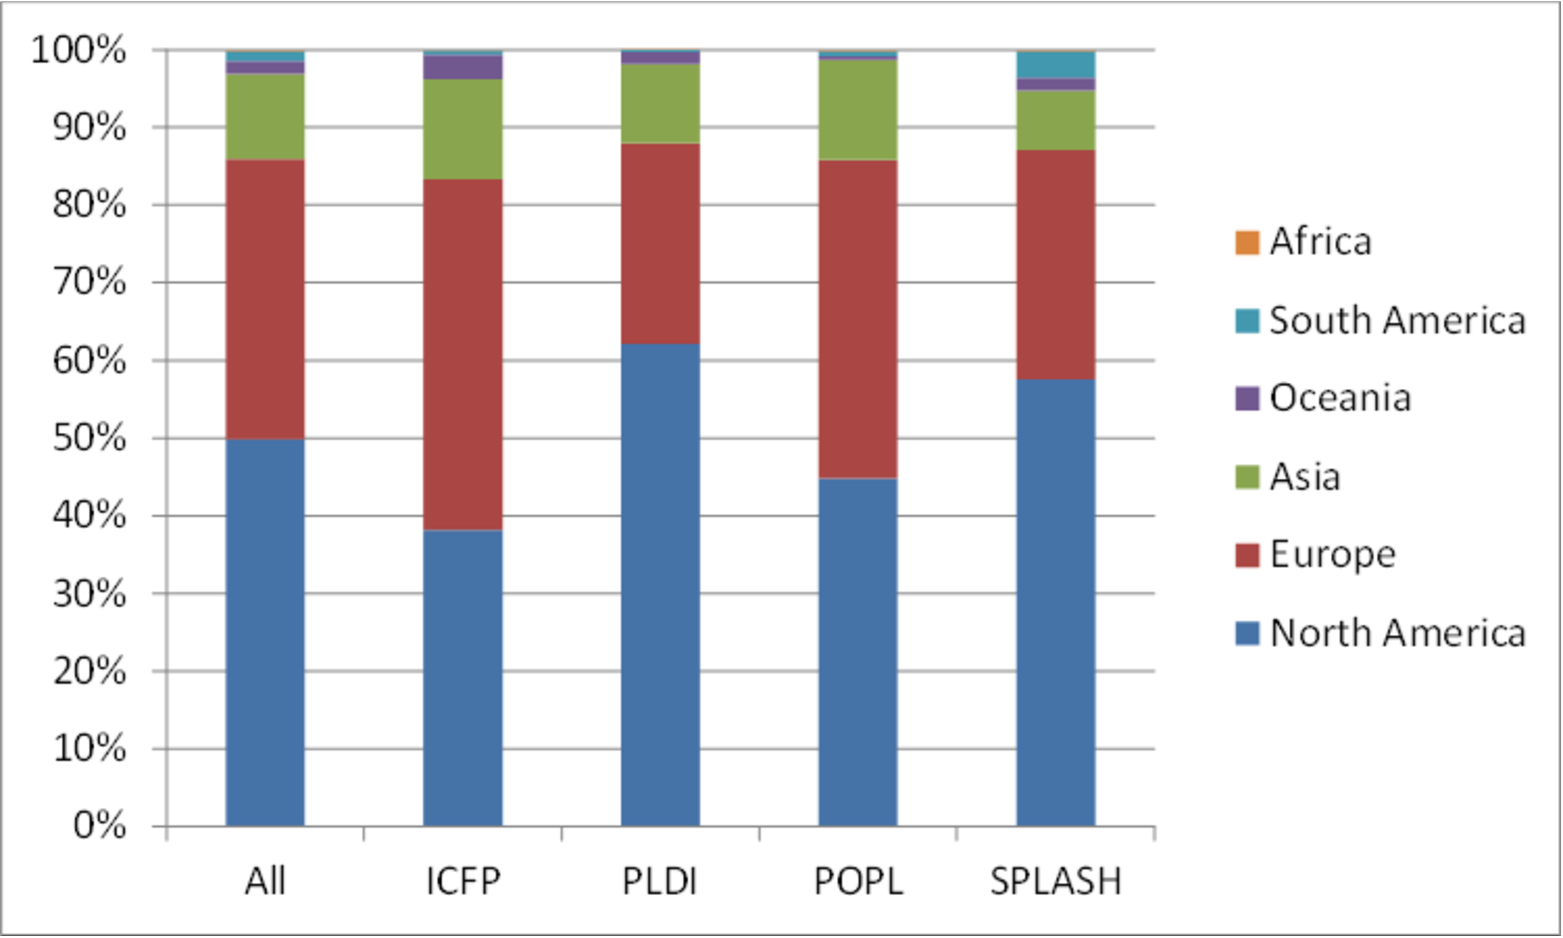
\includegraphics[width=0.7\textwidth]{ParticipantsOrigin.pdf}
  \caption{Overall origin of participants per conference.}
  \label{fig:demo-per-conf}
\end{figure}

\begin{table}
  \csvautotabular{../../output/sigplan/demographic_per_conf.csv}
\caption{For each kind of conference, distribution of participants per continent of origin}
\label{table:demo-per-conf}
\end{table}


Table~\ref{fig:demo-per-conf} and Figure~\ref{fig:demo-per-conf} show where all
participants came from. For each conference, we depict the distribution of
attendance per continent. Table~\ref{fig:demo-per-conf} also shows the portion
of attendants originating from the same continent as the one the event took
place in. To a first approximation, maximizing this last metric, i.e. hosting
conferences in the continent containing the majority of its community, is a
first simple heuristic to consider.

Taken as a whole, these conferences attracted 50\% participants from North
America, 36\% from Europe, 11\% from Asia, 2\% from Oceania, 1\% from South
America, and less than 0.2\% from Africa.
This data also emphasizes the relative anchor to a specific continent each
conference may have.
Most notably, PLDI and SPLASH appear to be very North
American-centric, while ICFP's core community seems to have a quite strong
anchor in Europe as well.

\begin{table}
  \csvautotabular{../../output/sigplan/demographic.csv}
  \caption{For each \event, continent in which it took place and distribution of
    each continent by origin of participants. The final column indicates the
    portion of participants that traveled from the same continent the
    conference took place in.}
  \label{table:demo-per-event}
\end{table}

\begin{figure}
  \centering
  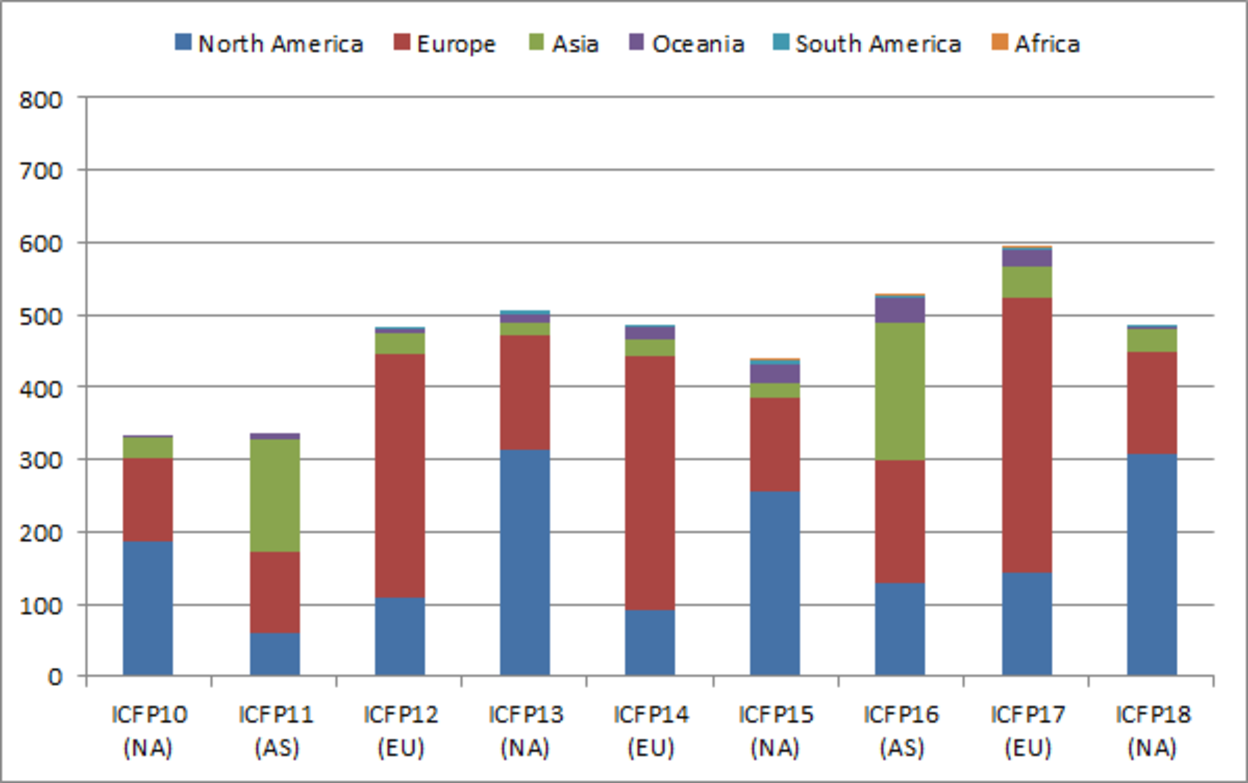
\includegraphics[width=0.45\textwidth,height=1.8in]{ParticipantsOriginICFP.pdf}
  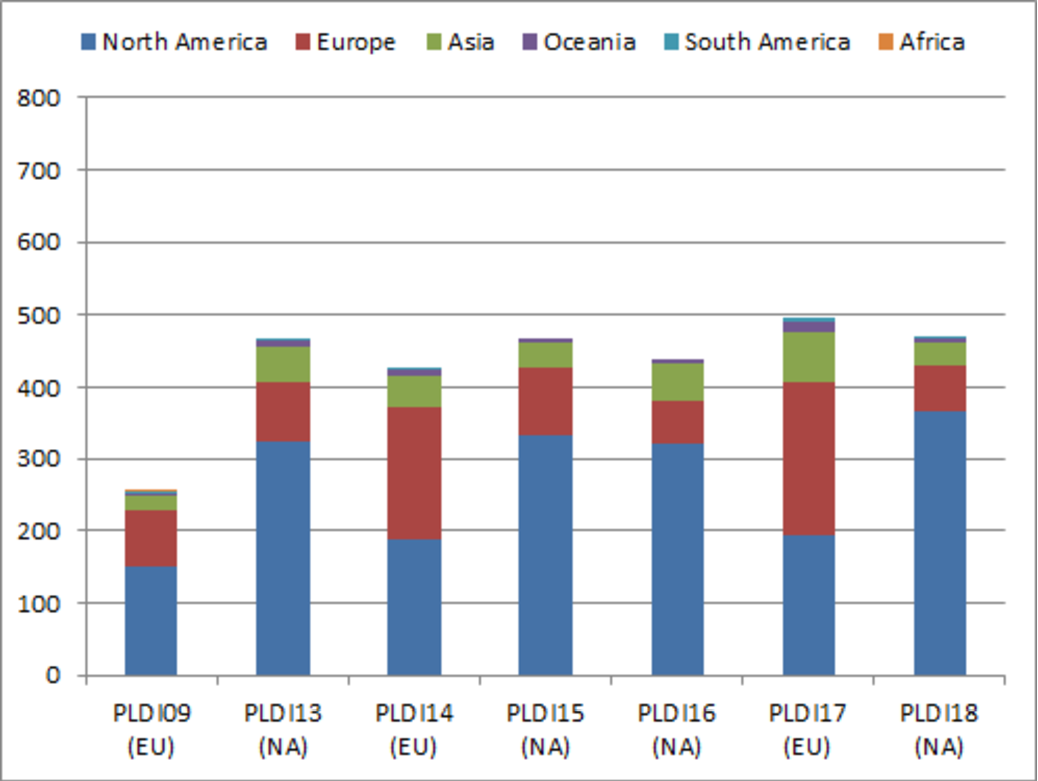
\includegraphics[width=0.45\textwidth,height=1.8in]{ParticipantsOriginPLDI.pdf}
  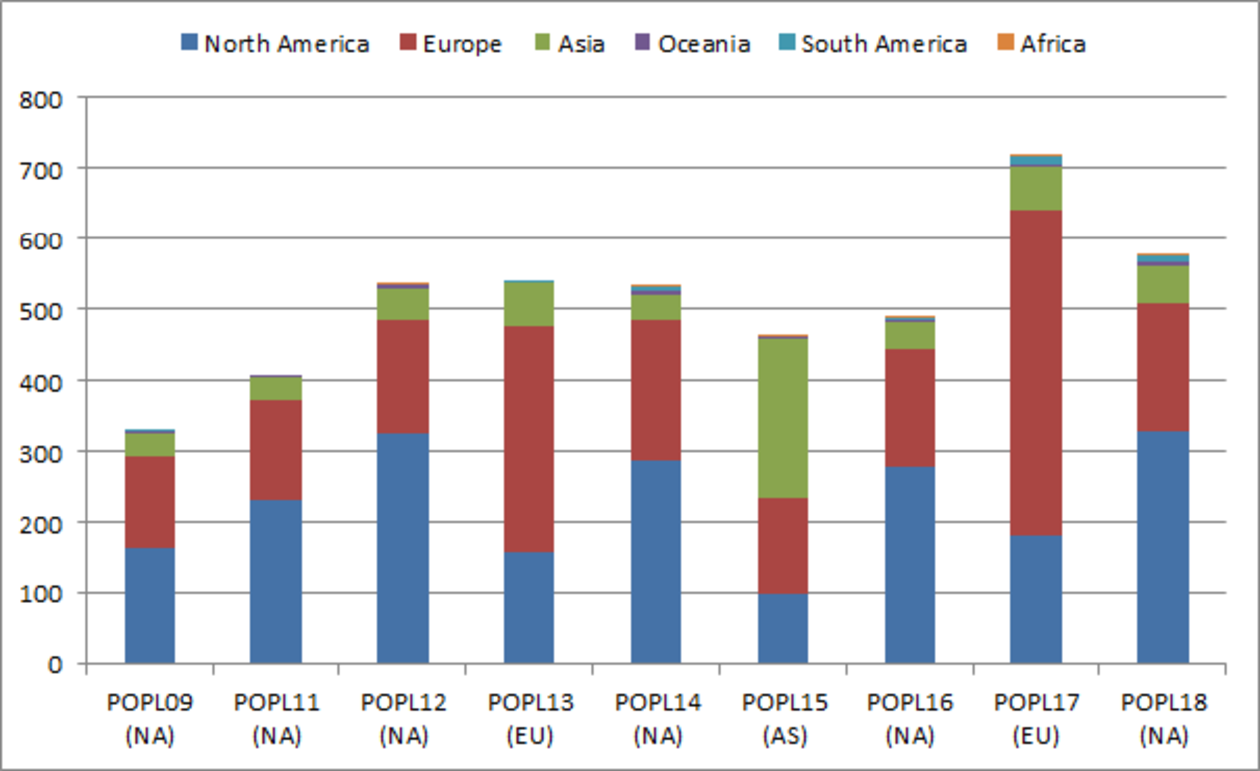
\includegraphics[width=0.45\textwidth,height=1.8in]{ParticipantsOriginPOPL.pdf}
  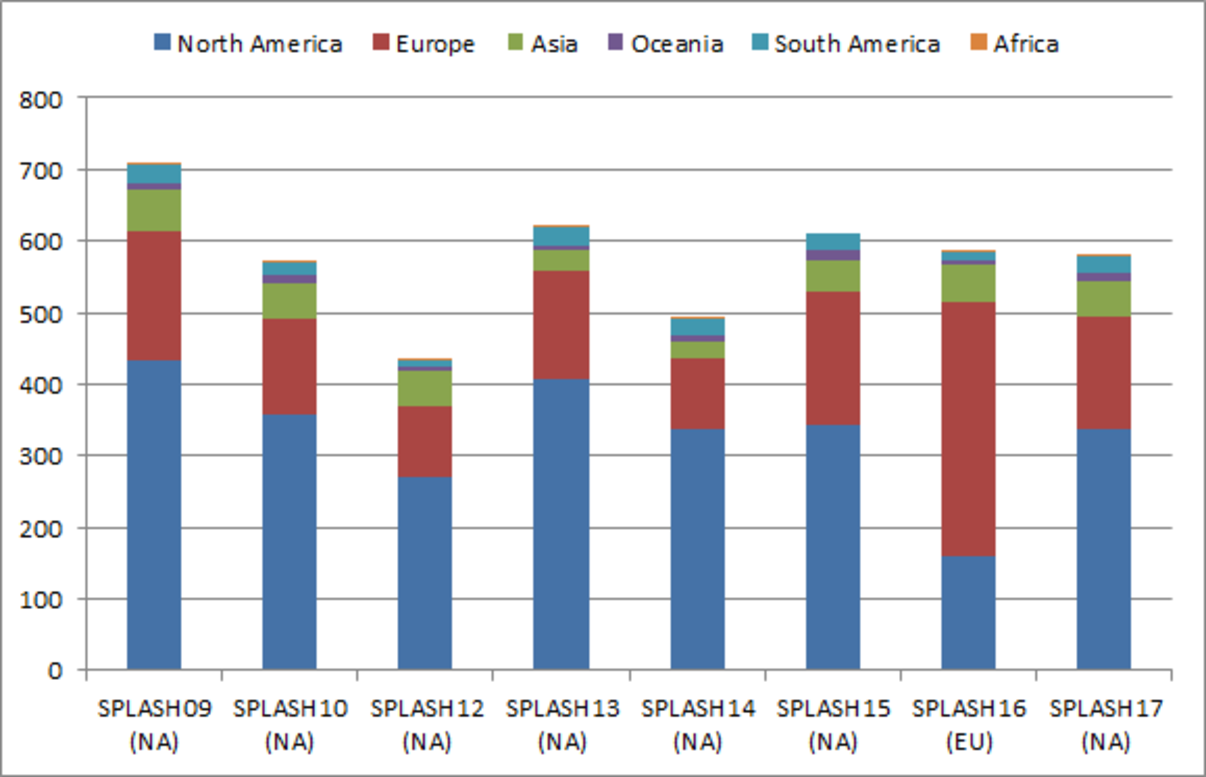
\includegraphics[width=0.45\textwidth,height=1.8in]{ParticipantsOriginSPLASH.pdf}
  \caption{Origin of participants for each conference, detail.}
  \label{fig:demo-per-event}
\end{figure}

This overall picture, however, hides some interesting facts pertaining to the
relationship between the conferences' locations and the origin of the participants.
Indeed, aggregating the attendance per conference intrinsically rests upon the
assumption of a uniform community attending each instance of the conference
every year. Table~\ref{fig:demo-per-event} and Figure~\ref{fig:demo-per-event}
show a more detailed breakdown of the origin of participants for each
conference, showing also the geographic region where the conferences were held.

These charts make it clear that the location of the conferences had a
substantial effect on attracting people from the same geographic areas. That
effect is quite visible for ICFP and POPL, with noticeable ups and downs of the
colored bars between North American and European participants when the
conferences were located in North America and Europe, respectively. Most
strikingly, Asian participation during POPL '15, ICFP '11 and ICFP '16, events
that took place on the Asian continent, is significantly higher than usual:
there appears to be a strong locality phenomenon. Crossing this data with
Table~\ref{table:footprint}, one can also notice that the only time SPLASH took
place in Europe turned out to be the least expensive edition, challenging our
previous observation that the conference appears to be mostly north
American-centric.

\begin{table}
  \csvautotabular{../../output/sigplan/demographic_delta.csv}
\caption{Geographical distribution of participation conditioned by the location of the \event}
\label{fig:local_effect}
\end{table}

Table~\ref{fig:local_effect} attempts to measure this locality effect. The
table depicts, all conferences being considered at once, the geographical
distribution of attendance conditioned by the geographical location of the
\event. The Asian phenomenon previously hinted at is here extremely
apparent: while overall on average, 10.9\% of the participants come from Asia,
this number is roughly multiplied by a factor 4 when the \event takes place in Asia --
without any significant drop in total volume of attendance that could indirectly bump
the percentage.
But interestingly, this phenomenon also exists in the case of Europe (+22.29\%
deviation to the average) and North America (+12.15\% deviation to the average).
Despite their name, international conferences appear to exhibit a fairly strong
local component.

Overall, this data shows that the goal of geographic inclusion was,
indeed, accomplished by organizing the conferences in diverse geographic areas
of the world. It also places Figure~\ref{fig:continents} into a broader context:
a naive interpretation of that chart might lead us to conclude that North
America and Europe are where most of this community is, but it is not that
simple. Because of the regional effect on participation, the distribution of
participants also reflects the fact that most of these conferences were held in
North America and Europe (30), only a few were held in Asia (3), and none was
held in South America, Oceania, or Africa.

The situation may be summed up into the following two elementary observations. 
\begin{obs}
  The vast majority of participants are split between North America and Europe,
  Asia to a much lesser degree. SPLASH and PLDI are strongly anchored in North
  America, ICFP and POPL fairly equally split between North America and Europe.
  \label{obs:dist-naive}
\end{obs}
This distribution however turns out to be \emph{strongly} dependent on the
location of the \event.
\begin{obs}
  There is a major ``locality" effect: it is both true that locality attract
  new participants, and distance repels some participants.
  \label{obs:locality}
\end{obs}

\subsection{Attendance overlaps}
\label{subsec:overlap}

Section~\ref{subsec:demo}, through the study of the demographic distribution of
attendance, has suggested the existence of local communities that only
partake in conferences when they take place close to their place of residency.
One can conversely look for groups of regular attendees, that participate to a given \conf
regardless of the location it is held in.

\begin{figure}
\centering
     \begin{subfigure}[b]{0.4\textwidth}
       \centering
       \csvautotabular{../../output/sigplan/overlap_intra_conf_POPL.csv}
       \caption{Case of POPL}
     \end{subfigure}
     \hfill
     \begin{subfigure}[b]{0.4\textwidth}
       \centering
       \csvautotabular{../../output/sigplan/overlap_intra_conf_ICFP.csv}
       \caption{Case of ICFP}
    \end{subfigure}

     \caption{For any two years, percentage of overlap in attendance at the corresponding editions of a conference (part 1)}
     \label{fig:overlap-conf-alpha}
\end{figure}

\begin{figure}
\centering
     \begin{subfigure}[b]{0.4\textwidth}
       \centering
       \csvautotabular{../../output/sigplan/overlap_intra_conf_PLDI.csv}
       \caption{Case of PLDI}
     \end{subfigure}
     \begin{subfigure}[b]{0.4\textwidth}
       \centering
       \csvautotabular{../../output/sigplan/overlap_intra_conf_SPLASH.csv}
       \caption{Case of SPLASH}
     \end{subfigure}

     \caption{For any two years, percentage of overlap in attendance at the corresponding editions of a conference (part 2)}
     \label{fig:overlap-conf-beta}
\end{figure}

Figures~\ref{fig:overlap-conf-alpha}~and~\ref{fig:overlap-conf-beta} present one
way to gather intuition about the reality and size of this phenomenon. For a
given conference at a time, we depicts, for any pair of years, the percentage of
attendees that participated in both events. In particular for two consecutive
years, this number oscillate between 15\% and 30\%. The vast majority of
participants of a conference were therefore not part of the previous edition.

\yz{TODO: This data is not striking enough and takes a lot of space. To aggregate
  more, or ditch in favor of the following tables only}\bcp{IMO it is worth
  keeping.  But maybe it could be moved later?}

\begin{figure}
  \centering
  \begin{subfigure}[b]{0.3\textwidth}
    \centering
    \csvautotabular{../../output/sigplan/overlap_cross_conf_ICFP_POPL.csv}
    \caption{POPL and ICFP}
  \end{subfigure}
  \begin{subfigure}[b]{0.3\textwidth}
    \centering
    \csvautotabular{../../output/sigplan/overlap_cross_conf_POPL_PLDI.csv}
    \caption{POPL and PLDI}
  \end{subfigure}
  \begin{subfigure}[b]{0.3\textwidth}
    \centering
    \csvautotabular{../../output/sigplan/overlap_cross_conf_POPL_SPLASH.csv}
    \caption{POPL and SPLASH}
  \end{subfigure}
  \begin{subfigure}[b]{0.3\textwidth}
    \centering
    \csvautotabular{../../output/sigplan/overlap_cross_conf_ICFP_PLDI.csv}
    \caption{ICFP and PLDI}
  \end{subfigure}
  \begin{subfigure}[b]{0.3\textwidth}
    \centering
    \csvautotabular{../../output/sigplan/overlap_cross_conf_ICFP_SPLASH.csv}
    \caption{ICFP and SPLASH}
  \end{subfigure}
  \begin{subfigure}[b]{0.3\textwidth}
    \centering
    \csvautotabular{../../output/sigplan/overlap_cross_conf_PLDI_SPLASH.csv}
    \caption{PLDI and SPLASH}
  \end{subfigure}
   \caption{For every year, overlap in attendance between the events of two
     different conferences\bcp{Maybe we could also have an aggregate count
       for each pair, showing how many people {\em ever} went to both (even
       in different years).}}
  \label{fig:overlap-cross}
\end{figure}

Arguably more useful for practical purposes is to evaluate the overlap 
between the events for the same year of two different conferences.
Figure~\ref{fig:overlap-cross} depicts this data for any pairing of the four
conferences considered. The overlap is strikingly low for most conferences.

\begin{figure}
  \csvautotabular{../../output/sigplan/number_of_participations.csv}
\caption{Overall and for each conference, the average number of instances a
  participant has taken part of, and the percentage of them that has
  attended at least $k$ instances, for $k\in\llbracket 2 \dots 5
  \rrbracket$. Remark: the means and percentages are here computed with
  respect to \emph{unique} participants.  \bcp{I really like this table.}}
\label{fig:reccurent}
\end{figure}

\begin{figure}
  \centering
  \begin{subfigure}[b]{0.4\textwidth}
    \centering
    \csvautotabular{../../output/sigplan/old_timer_POPL.csv}
    \caption{Case of POPL}
  \end{subfigure}
  \begin{subfigure}[b]{0.4\textwidth}
    \centering
    \csvautotabular{../../output/sigplan/old_timer_ICFP.csv}
    \caption{Case of ICFP}
  \end{subfigure}
  \\
  \begin{subfigure}[b]{0.4\textwidth}
    \centering
    \csvautotabular{../../output/sigplan/old_timer_PLDI.csv}
    \caption{Case of PLDI}
  \end{subfigure}
  \begin{subfigure}[b]{0.4\textwidth}
    \centering
    \csvautotabular{../../output/sigplan/old_timer_SPLASH.csv}
    \caption{Case of SPLASH}
  \end{subfigure}
  \caption{For each conference, percentage of participants that have been
    part of a previous edition of the same conference \bcp{Is this sort of
      the same information as Figure 8?}}
  \label{fig:old-timers}
\end{figure}

Finally, Figure~\ref{fig:reccurent} and \ref{fig:old-timers} offer two different views on reccurent participations. Figure~\ref{fig:reccurent} represents respectively for the whole dataset and for each conference individually the average number of editions an average participant has been part of, as well as the percentage of participants that has been part of at least some amount of times. We immediately remark that no less than 75\% of unique participants has been part of a single edition.
Figure~\ref{fig:old-timers} represents for each instance of each conference the percentage of participants that has participated in a previous instance of the conference, among our dataset.

